\subsection{Atención textual: AttnGAN}
AttnGAN representa una evolución respecto a la cGAN, especialmente en cuanto a estabilidad durante el entrenamiento y eficiencia en la gestión de recursos computacionales. A diferencia de las cGANs implementadas en TensorFlow, AttnGAN se desarrolló sobre PyTorch, lo que permitió un mayor control sobre la asignación de memoria y una mejor capacidad para manejar grandes volúmenes de datos. Este modelo está específicamente diseñado para generar imágenes a partir de descripciones textuales mediante el uso de mecanismos de atención, que permiten asociar palabras o fragmentos específicos del texto con regiones concretas de la imagen. Este enfoque favorece una mayor coherencia semántica entre el contenido textual y visual, y mejora el nivel de detalle generado en las imágenes.

\subsubsection{Configuración del Entrenamiento}
El modelo fue entrenado utilizando el dataset COCO completo, el cual proporciona una gran variedad de imágenes junto con múltiples descripciones por imagen, lo que resulta ideal para tareas de generación condicionada por texto. Gracias a la eficiencia de PyTorch en la gestión de memoria, no fue necesario trabajar con subconjuntos del dataset, como sí ocurrió en el caso de la cGAN. El entrenamiento se realizó en la plataforma Kaggle, que ofrece acceso gratuito a GPU pero impone una limitación de 30 horas semanales de ejecución. Esta restricción obligó a limitar el entrenamiento a un máximo de 40 épocas por ejecución completa.

A pesar de esta limitación temporal, la estabilidad del entrenamiento fue notable. PyTorch permitió mantener un tamaño de batch razonable sin generar errores de memoria, lo que favoreció una convergencia progresiva y consistente. Asimismo, el modelo integra mecanismos de atención en múltiples niveles: en cada etapa del proceso generativo, el sistema aprende a enfocar su atención en las partes más relevantes de la descripción textual, optimizando así la correspondencia entre texto e imagen.

\subsubsection{Proceso de Entrenamiento}
El entrenamiento de AttnGAN se dividió en varias fases, cada una diseñada para evaluar y refinar la calidad de las imágenes generadas. Aunque el límite de 40 épocas restringía el alcance del entrenamiento, fue posible observar una mejora progresiva en la correspondencia entre texto e imagen. En comparación con la cGAN, donde la pérdida era altamente inestable, AttnGAN mostró una evolución más suave y coherente, aunque no se generaron curvas de pérdida formales para su análisis.

En ausencia de métricas cuantitativas detalladas, se utilizó una estrategia de evaluación visual para examinar las imágenes generadas a lo largo del entrenamiento. Esta evaluación permitió ajustar los hiperparámetros, como la tasa de aprendizaje y la arquitectura de las capas intermedias, en función de la calidad perceptual observada. En futuras implementaciones, contar con un sistema de logging más completo permitiría extraer información cuantitativa útil para complementar esta evaluación.

\subsubsection{Resultados y Evaluación Visual}
A nivel de resultados, AttnGAN logró generar imágenes que reflejaban de forma razonable la estructura y elementos clave descritos en el texto. Sin embargo, las imágenes seguían presentando borrosidad y falta de precisión en los detalles, especialmente en contextos con múltiples objetos o relaciones espaciales complejas. La Figura \ref{fig:attn} muestra la mejor imagen obtenida durante el entrenamiento: aunque transmite la intención general del texto de entrada, la baja resolución y la ambigüedad visual limitan su aplicabilidad en escenarios que requieran imágenes de alta fidelidad.

\begin{figure}[H]
\centering
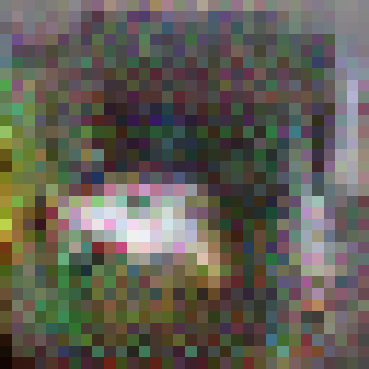
\includegraphics[width=0.4\textwidth]{generated_image_epoch_10}
\caption{Mejor imagen generada por AttnGAN durante el entrenamiento.}
\label{fig:attn}
\end{figure}

\subsubsection{Conclusión}
AttnGAN superó las limitaciones observadas en la cGAN, particularmente en términos de estabilidad del entrenamiento y manejo de memoria. La capacidad de trabajar con el dataset COCO completo y la integración de mecanismos de atención ofrecieron una mejora sustancial en la correspondencia semántica entre descripciones textuales e imágenes generadas. Sin embargo, el rendimiento visual aún se vio limitado por la duración del entrenamiento y las restricciones del entorno de ejecución. En condiciones con mayor disponibilidad de recursos computacionales, sería posible extender el número de épocas y optimizar aún más la calidad de las imágenes producidas.
